\begin{figure}[t!]
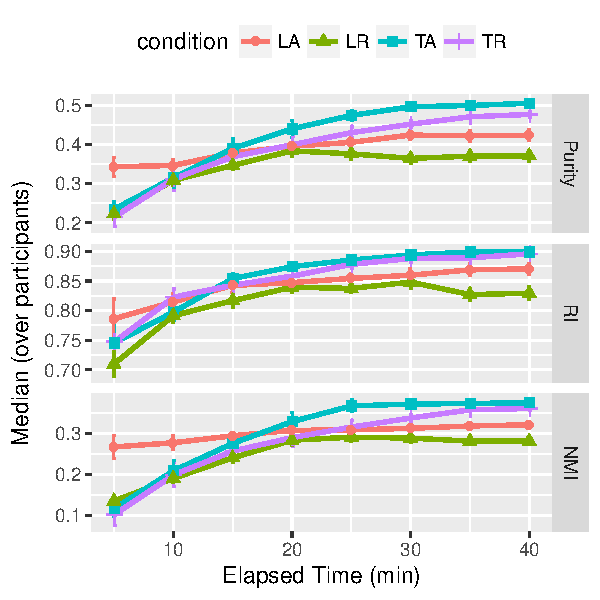
\includegraphics[width=\linewidth]{2016_acl_doclabel/auto_fig/user_exp_plot}
\caption{User study results on \abr{us} Congressional Bills dataset. Active learning selection helps initially, but the combination of active learning selection and topic model overview has highest quality labels by the end of the task.}
\label{fig:results}
\end{figure}

Following the synthetic experiments, we conduct a user study with
forty participants to evaluate \name{} (\abr{ta} condition) against
three alternatives that lack topic overview (\abr{la}), active
learning selection (\abr{tr}), or both (\abr{lr}) (Sections~\ref{sub:procedures} and~\ref{sub:cluster_results}). Then, we conduct a crowdsourced study to compare the overall effectiveness of the label set generated by the participants in the four conditions (Section~\ref{sub:label_results}).

\subsection{Method}
\label{sub:procedures}

We use the freelance marketplace Upwork to recruit online
participants.\footnote{
\let\hyper@linkurl\saved@hyper@linkurl
\url{http://Upwork.com}\NoHyper} We require participants to have
more than $90\%$ job success on Upwork, English fluency, and \abr{us}
residency. Participants are randomly assigned to one of the four conditions and
we recruited ten participants per condition.

Participants completed a demographic questionnaire, viewed a video of task
instructions, and then interacted with the system and labeled documents until
satisfied with the labels or forty minutes had elapsed.\footnote{Forty minutes
  of activity, excluding system time to classify and update
  documents. Participants nearly exhausted the time: $39.3$
 average minutes in \abr{ta}, $38.8$ in \abr{tr}, $40.0$ in \abr{la}, and $35.9$ in
  \abr{lr}.} The session ended with a survey, where participants rated mental,
physical, and temporal demand, and performance, effort, and frustration on
20-point scales, using questions adapted from the \abr{nasa} Task Load
Index~\cite[\abr{tlx}]{hart1988development}. The survey also included 7-point
scales for ease of coming up with labels, usefulness and satisfaction with the
system, and---for \abr{tr} and \abr{ta}---topic information helpfulness. Each
participant was paid fifteen dollars.\footnote{User study data available at
\let\hyper@linkurl\saved@hyper@linkurl
  \url{http://github.com/Pinafore/publications/tree/master/2016_acl_doclabel/data/user_exp}
  \NoHyper
  }

For statistical analysis, we primarily use $2\times2$ (\emph{overview} $\times$
\emph{selection}) \abr{anova}s with Aligned Rank
Transform~\cite[\abr{art}]{wobbrock2011aligned}, which is a non-parametric
alternative to a standard \abr{anova} that is appropriate when data are not
expected to meet the normality assumption of \abr{anova}.
















\subsection{Document Cluster Evaluation}
\label{sub:cluster_results}





We analyze the data by dividing the forty-minute labeling task into
five minute intervals. If a participant stopped before the time
limit, we consider their final dataset to stay the same for any
remaining intervals. Figure~\ref{fig:results} shows the
measures across study conditions, with similar trends for all three
measures.

\paragraph{Topic model overview and active learning both significantly improve final dataset measures.}

The topic overview and active selection conditions significantly
outperform the list overview and random selection, respectively, on
the final label quality metrics. Table~\ref{tab:stats} shows the
results of separate $2\times2$ \abr{anova}s with \abr{art} with each
of final purity, \abr{ri}, and \abr{nmi} scores. There are significant main
effects of \emph{overview} and \emph{selection} on all three metrics;
no interaction effects were significant.






\begin{table}[t!]
\small
\resizebox{\columnwidth}{!}{
\begin{tabular}{*5c}
    \hline
    & \multicolumn{2}{c}{$F$} & \multicolumn{2}{c}{$p$} \\
    & Overview & Selection & Overview & Selection
    \tabularnewline \hline \hline
	final purity & 81.03& 7.18 & $< .001$ & $.011$
    \tabularnewline
    \hline
	final \abr{ri} & 39.89 & 6.28 &  $<.001$ & $.017$
\tabularnewline
\hline
	final \abr{nmi} &70.92 &9.87 & $<.001$ & $.003$
 \tabularnewline
\hline
	\multicolumn{5}{c}{df(1,36) for all reported results}
\end{tabular}
}
\caption{Results from $2\times2$ \abr{anova} with \abr{art} analyses on the
final purity, \abr{ri}, and \abr{nmi} metrics. Only main effects for
the factors of \emph{overview} and \emph{selection} are shown; no interaction
effects were statistically significant.  Topics and active learning
both had significant effects on quality scores.}
\label{tab:stats}
\end{table}

\paragraph{\abr{tr} outperforms \abr{la}.}

Topic models by themselves outperform traditional active learning
strategies (Figure~\ref{fig:results}).  \abr{la} performed
better than \abr{lr}; while active learning was useful, it was not as
useful as the topic model overview (\abr{tr} and \abr{ta}).





\paragraph{\abr{la} provides an initial benefit.}

Average purity, \abr{nmi} and \abr{ri} were highest with \abr{la} for
the earliest labeling time intervals.  Thus, when time is very
limited, using traditional active learning (\abr{la}) is preferable to
topic overviews; users need time to explore the topics and a subset of
documents within them. Table~\ref{tab:early_results} shows the metrics
after ten minutes. Separate $2\times2$ \abr{anova}s with \abr{art} on
the means of purity, \abr{nmi} and \abr{ri} revealed a significant
interaction effect between \emph{overview} and \emph{selection} on
mean \abr{nmi} ($F(1,36)= 5.58$, $p$ = $.024$), confirming the early
performance trends seen in Figure~\ref{fig:results} at least for
\abr{nmi}. No other main or interaction effects were significant,
likely due to low statistical power.

\begin{table}[t!]
\small
\resizebox{\columnwidth}{!}{
\begin{tabular}{*4c}
    \hline
    & \multicolumn{3}{c}{$M \,\,\pm\,\, SD \,[median]$} \\
    &purity & \abr{ri} & \abr{nmi}
    \tabularnewline \hline \hline
	\abr{ta} & $0.31 \,\pm\, 0.08 \,[0.32]$& $0.80 \,\pm\, 0.05 \,[0.80]$ & $0.19 \,\pm\, 0.08 \,[0.21]$
    \tabularnewline
    \hline
	\abr{tr} & $0.32 \,\pm\, 0.09 \,[0.31]$& $0.82 \,\pm\, 0.04 \,[0.82]$ &  $0.21 \,\pm\, 0.09 \,[0.20]$
\tabularnewline
\hline
	\abr{la} &$0.35 \,\pm\, 0.05 \,[0.35]$ & $0.82 \,\pm\, 0.04 \,[0.81]$ & $0.27 \,\pm\, 0.05 \,[0.28]$
 \tabularnewline \hline
	\abr{lr} &$0.31 \,\pm\, 0.04 \,[0.31]$ &$0.79 \,\pm\, 0.04 \,[0.79]$ & $0.19 \,\pm\, 0.03 \,[0.19]$
	 \tabularnewline \hline
\end{tabular}
}
\caption{Mean, standard deviation, and median purity, \abr{ri}, and \abr{nmi}
  after ten minutes. \abr{nmi} in particular shows the benefit of \abr{la} over other conditions at early time intervals.}
\label{tab:early_results}
\end{table}



\begin{table*}[t!]
\resizebox{\textwidth}{!}{
\begin{tabular}{*7c}
    \hline
        & \multicolumn{6}{c}{$M \,\,\pm\,\, SD \,[median]$} \\
    Condition & Mental Demand & Physical Demand & Temporal Demand & Performance & Effort & Frustration
    \tabularnewline \hline \hline
	\abr{ta} &$9.8 \,\,\pm\,\, 5.6 \,[10]$&$2.9 \,\,\pm\,\, 3.4 \,[2]$&$9 \,\,\pm\,\, 7.8 \,[7$]&$5.5 \,\,\pm\,\, 5.8 \,[1.5]$&$9.4 \,\,\pm\,\, 6.3 \,[10]$&$4.5 \,\,\pm\,\, 5.5 \,[1.5]$

    \tabularnewline
    \hline
	\abr{tr} &$10.6 \,\,\pm\,\, 4.5 \,[11]$&$2.4 \,\,\pm\,\, 2.8 \,[1]$&$7.4 \,\,\pm\,\, 4.1 \,[9]$&$8.8 \,\,\pm\,\, 6.1 \,[7.5]$&$9.8 \,\,\pm\,\, 3.7 \,[10]$&$3.9 \,\,\pm\,\, 3.0 \,[3.5]$

\tabularnewline
\hline
	\abr{la} &$9.1 \,\,\pm\,\, 5.5 \,[10]$&$1.7 \,\,\pm\,\, 1.3 \,[1]$&$10.2 \,\,\pm\,\, 4.8 \,[11]$&$8.6 \,\,\pm\,\, 5.3 \,[10]$&$10.7 \,\,\pm\,\, 6.2 \,[12.5]$&$6.7 \,\,\pm\,\, 5.1 \,[5.5]$

 \tabularnewline
\hline
	\abr{lr} &$9.8 \,\,\pm\,\, 6.1 \,[10]$&$3.3 \,\,\pm\,\, 2.9 \,[2]$&$9.3 \,\,\pm\,\, 5.7 \,[10]$&$9.4 \,\,\pm\,\, 5.6 \,[10]$&$9.4 \,\,\pm\,\, 6.2 \,[10]$&	$7.9 \,\,\pm\,\, 5.4 \,[8]$
 \tabularnewline
\hline
\end{tabular}
}
\caption{
Mean, standard deviation, and median results from \abr{nasa-tlx}
 post-survey. All questions are scaled 1 (low)--20 (high), except performance, which is scaled 1 (good)--20 (poor). Users found topic model overview conditions, \abr{tr} and \abr{ta}, to be significantly less frustrating than the list overview conditions.}
\label{tab:NASA_res}
\end{table*}

\paragraph{Subjective ratings.}

Table~\ref{tab:NASA_res} shows the average scores given for the six
\abr{nasa-tlx} questions in different conditions. Separate $2\times2$
\abr{anova} with \abr{art} for each of the measures revealed only one
significant result: participants who used the topic model overview find the
task to be significantly less frustrating (\mbox{$M=4.2$} and \mbox{$median=2$})
than those who used the list overview (\mbox{$M=7.3$} and \mbox{$median=6.5$})
on a scale from 1 (low frustration) to 20 (high frustration)
(\mbox{$F(1,36)=4.43$}, \mbox{$p=.042$}), confirming that the topic overview
helps users organize their thoughts and experience less stress during labeling.

Participants in the \abr{ta} and \abr{tr} conditions rate topic
information to be useful in completing the task (\mbox{$M=5.0$} and
\mbox{$median=5$}) on a scale from 1 (not useful at all) to 7 (very
useful).  Overall, users were positive about their experience with the
system. Participants in all conditions rated overall satisfaction
with the interface positively (\mbox{$M=5.8$ and $median=6$}) on a
scale from 1 (not satisfied at all) to 7 (very satisfied).
\paragraph{Discussion}

One can argue that using topic overviews for labeling could have a negative effect:
users may ignore the document content and focus on topics for labeling. We tried
to avoid this issue by making it clear in the instructions that they need to
focus on document content and use topics as a guidance. On average, the participants in
\abr{tr} created 1.96 labels per topic and the participants in \abr{ta} created
2.26 labels per topic. This suggests that participants are going beyond what
they see in topics for labeling, at least in the \abr{ta} condition.









\subsection{Label Evaluation Results}
\label{sub:label_results}

Section~\ref{sub:cluster_results} compares clusters of documents in different
conditions against the gold clustering but ignores what the labels
actually are. To assess how the final induced label sets compare in
different conditions, we use crowdsourcing to assess the quality of
documents' labels.  

For completeness, we also compare labels against a fully automatic
labeling method~\cite{aletras2014labelling} that does not require
human intervention.  We assign \emph{automatic} labels to documents
based on their most prominent topic.

We ask users on a crowdsourcing platform to \emph{vote} for the ``best'' and
``worst'' label that describes the content of a \abr{us} congressional
bill (we use Crowdflower and require contributors to be in the \abr{us}).

Five users label each document and we use the aggregated results generated by
Crowdflower. The user gets \$0.20 for each task. 

We randomly choose $200$ documents from our dataset (Section
\ref{sub:data}). For each chosen document, we randomly choose a participant from
all four conditions (\abr{ta}, \abr{tr}, \abr{la}, \abr{lr}). The labels
assigned in different conditions and the automatic label of the document's prominent
topic construct the candidate labels for the document.\footnote{Some
  participants had typos in the labels. We corrected all the typos using
  pyEnchant (\let\hyper@linkurl\saved@hyper@linkurl \url{http://pythonhosted.org/pyenchant/} \NoHyper) spellchecker. If the
  corrected label was still wrong, we corrected it manually.} Identical labels are
merged into one label to avoid showing duplicate labels to users. If a merged
label gets a ``best'' or ``worst'' vote, we split that vote across all the
identical instances.\footnote{
Evaluation data available at \let\hyper@linkurl\saved@hyper@linkurl\url{http://github.com/Pinafore/publications/tree/master/2016_acl_doclabel/data/label_eval} \NoHyper
}
Figure~\ref{fig:eval_votes} shows the average number of ``best'' and ``worst''
votes for each condition and the automatic method.
\name{} (\abr{ta}) receives the most ``best'' votes and the fewest
``worst'' votes. \abr{lr} receive the most worst votes. The automatic labels, interestingly, appear to do at least as well as the list view labels, with a similar number of best votes and fewer worst votes.  This indicates that automatic labels have reasonable quality compared to at least some manually generated labels. However, when users are provided with topic model overview, with or
without active learning selection, they can generate label sets that
 improve upon automatic labels and labels assigned without the topic
model overview.













\begin{figure}[t!]
 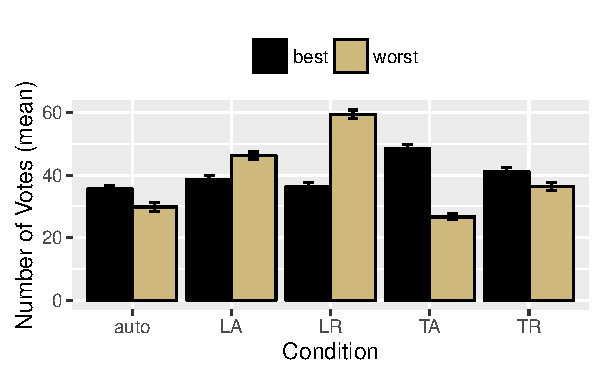
\includegraphics[width=0.5\textwidth]{2016_acl_doclabel/auto_fig/eval_votes}
 \caption{Best and worst votes for document labels. Error
   bars are standard error from bootstrap sample. \name{}
   (\abr{ta}) gets the most best votes and the fewest worst votes.}
\label{fig:eval_votes}
\end{figure}